%
% beamerExample.tex
% 
% Copyright 2013 Benjamin Tovar Cisneros <benjamin.tovarcis@gmail.com>
% 
% This program is free software; you can redistribute it and/or modify
% it under the terms of the GNU General Public License as published by
% the Free Software Foundation; either version 2 of the License, or
% (at your option) any later version.
% 
% This program is distributed in the hope that it will be useful,
% but WITHOUT ANY WARRANTY; without even the implied warranty of
% MERCHANTABILITY or FITNESS FOR A PARTICULAR PURPOSE.  See the
% GNU General Public License for more details.
% 
% You should have received a copy of the GNU General Public License
% along with this program; if not, write to the Free Software
% Foundation, Inc., 51 Franklin Street, Fifth Floor, Boston,
% MA 02110-1301, USA.
% 
% 
% ******************************************************************************
% LATEX PARAMETERS
% ******************************************************************************
% Tell LaTex that this document is using beamer 
\documentclass[xcolor=dvipsnames,mathserif]{beamer} 
% Color theme of the slides 
% TRY USING DIFFERENT RGB COLORS
\usecolortheme[RGB={70,130,180}]{structure} 
% Slides theme 
% CHECK THIS URL: http://www.math.umbc.edu/~rouben/beamer/quickstart-Z-H-30.html#node_tag_Temp_75
\usetheme{Dresden} 
% Links in slides settings
\definecolor{links}{HTML}{2A1B81}
\hypersetup{colorlinks,linkcolor=,urlcolor=links}
%% load source code package
\usepackage{listings}
%% Harvard bibliography style
\usepackage{natbib}
\bibpunct[:]{(}{)}{;}{a}{}{,}
% %% hyperreferences inside the slides
% \usepackage{hyperref}
% ******************************************************************************
% SLIDES PARAMETERS
% ******************************************************************************
\title{Random \LaTeX{} presentation using the Beamer class}
\subtitle{as a subtitle, \LaTeX{}  definitely rocks}
\author{Biotech. Benjamin Tovar Cisneros}
\institute{Bioinformatics Research Group @ ITESM campus Monterrey}
\date{\today}

\begin{document}
% Set background image with the Institution logo
\usebackgroundtemplate{
\includegraphics[width=0.7\textwidth]{images/format/logoTecTransparent2}}

%source code edition parameters
\lstset{
   breakatwhitespace=true,
   language=R,
   columns=fullflexible,
   keepspaces=true,
   breaklines=true,
   tabsize=3, 
   showstringspaces=false,
   extendedchars=true,
   numbers=left,
   numberstyle=\tiny,
   aboveskip=-40pt,
   frame=leftline,
   commentstyle=\itshape\color{gray},
}

% ******************************************************************************
% PRESENTATION FIRST PAGE
% ******************************************************************************
\frame{\titlepage}

% LOAD MYSELF.TEX
% ******************************************************************************
% INTRODUCING MYSELF 
% ******************************************************************************

\begin{frame}
\frametitle{Author's presentation}
\begin{columns}[c]
\column{2.5in}

\begin{itemize}
	\item Author's data:
	\begin{itemize}
		\item Your name
		\item Your academic grade | your school
	\end{itemize}
	\item Author's ascriptions:
	\begin{itemize}
		\item Your research unit 1 | University 1
		\item Your research unit 2 | University 2
	\end{itemize}
\end{itemize}

\column{1.5in}
% Add a photo of you
\framebox{
\includegraphics[width=1.5in]{images/format/linux_negro_gris}}
\end{columns}
\end{frame}


% ******************************************************************************
% INDEX
% ******************************************************************************
\section[Outline]{}
\frame{\tableofcontents}

% ******************************************************************************
% LOAD TEX FILES
% ******************************************************************************
\section{Intro} 

\subsection{Scope, Sense and Purpose}
\begin{frame}[t]
\frametitle{Introduction}
\framesubtitle{Sense -- Nonsense -- Madness}
\bigskip
\bigskip
\bigskip

\begin{columns}[t]
\begin{column}{.3\textwidth}
\textbf{Useful}\\[3mm]
\begin{itemize}
\item Articles
\item Books
\item Scientific papers
\item Applications
\end{itemize}
\end{column}
\begin{column}{.30\textwidth}
\textbf{Nonsense}\\[3mm]
\begin{itemize}
\item Private mail
\item Invitations to your birthday party
\item Drink Menu
\end{itemize}
\end{column}
\begin{column}{.3\textwidth}
\textbf{Madness}\\[3mm]
\begin{itemize}
\item Shopping list
\item Brainstorming
\item \ldots 
\end{itemize}
\end{column}
\end{columns}
\end{frame}

%-------------------------------------------------------------------------------

\begin{frame} 
\frametitle{From Code To Document}
\framesubtitle{No WYSIWYG} 
\begin{columns}
\begin{column}{.7\textwidth}
\image{\textwidth}{image/worddoc.jpg}{\textbf{W}hat \textbf{Y}ou \textbf{S}ee \textbf{I}s \textbf{W}hat \textbf{Y}ou
\textbf{G}et}{img:worddoc}
\end{column}
\begin{column}{.3\textwidth}
\image{\textwidth}{image/codescreen.png}{\textbf{W}hat \textbf{W}ill \textbf{I} \textbf{G}et?}{img:codescreen}
%% Compile Animation
\end{column}
\end{columns}
\end{frame}

%-------------------------------------------------------------------------------

\begin{frame}
\frametitle{Introduction}
\framesubtitle{Approach}
\begin{columns}[onlytextwidth]
\begin{column}{0.40\textwidth}
\image{.8\textwidth}{image/codescreen.png}{Text File with \LaTeX ~-Code}{img:code}
\end{column}
\begin{column}{0.25\textwidth}
\image{.8\textwidth}{image/miktex.jpg}{Compiler (z.B. MikTeX)}{img:miktex}
\end{column}
\begin{column}{0.25\textwidth}
\image{.6\textwidth}{image/pdflogo.png}{good-looking, legible and printable document}{img:pdf}
\end{column}
\end{columns}
\end{frame}


%-------------------------------------------------------------------------------

\subsection{Advantages \& Disadvantages}
\begin{frame}
\frametitle{Introduction}
\framesubtitle{Advantages \& Disadvantages}
Advantages
\begin{itemize}
\item  dynamic directories and references
\item  automated layouts
\item  simple distributed work
\end{itemize}
Disadvantages
\begin{itemize}
\item  What do I get in the end?
\item  many, partly complex commands
\end{itemize}
\end{frame}

%-------------------------------------------------------------------------------

\subsection{\LaTeX --Compiler}
\begin{frame}
\frametitle{Introduction}
\framesubtitle{\LaTeX - Compiler}
\begin{columns}[t]
\begin{column}{.4\textwidth}
\textbf{Software for Windows:}\\
\begin{itemize}
  \item MikTex (http://www.miktex.org)\\
   2 alternatives: Basic or  Complete
  \item ProTeXt (http://www.tug.org/protext)\\
contains MikTex, TeXnicCenter and Ghostscript – simple installation\\
\end{itemize}
\end{column}
\begin{column}{.6\textwidth}
\textbf{Software for *nix:}
\begin{itemize}
  \item TeXLive\\
Packages for Ubuntu: {\ttfamily texlive-full} is the full meta-package with all necessary packages. Also contains the following:
\begin{itemize}
  \item {\ttfamily texlive-base
  \item texlive-lang-german}
\end{itemize}
Installation: {\ttfamily sudo apt-get install texlive-full}
\item MacOS: MacTeX (http://www.tug.org/mactex/2009)\\
\end{itemize}
\end{column}
\end{columns}
\end{frame}

%-------------------------------------------------------------------------------

\subsection{Free Editors}

\subsubsection{*nix}
\begin{frame}
\frametitle{Introduction}
\framesubtitle{Free Editors -- Linus \& MacOS }
\begin{itemize}
 \item Kile\footnote{http://kile.sourceforge.net/}\\KDE-program, also usable under Gnome\slash Unity etc.
 Installation for Debian systemes with {\ttfamily sudo apt-get
 install kile}.
  \item Vim \LaTeX -suite (Plugin)\footnote{http://vim-latex.sourceforge.net/}\\
  Dream for Vim users.
  \item TexShop (MacOS)\footnote{http://pages.uoregon.edu/koch/texshop/}
\end{itemize}
\end{frame}

%-------------------------------------------------------------------------------

\subsubsection{Windows}
\begin{frame}
\frametitle{Introduction}
\framesubtitle{Free Editors -- Windows}
\begin{itemize}
\item TeXnicCenter\footnote{http://www.texniccenter.org/}
  %\item \ldots
\end{itemize}
\end{frame}

%-------------------------------------------------------------------------------

\subsubsection{Cross-Platform}
\begin{frame}
\frametitle{Introduction}
\framesubtitle{Free Editors -- Cross-Platform}
\begin{itemize}
  \item TeXMaker\footnote{http://www.xm1math.net/texmaker}\\
   Used in this turorial.
  \item TeXstudio\footnote{http://sourceforge.net/projects/texstudio/?source=dlp}\\
  Like TeXMaker, but more powerful.
  \item TeXlipse\footnote{http://texlipse.sourceforge.net/}\\ For advanced users, plugin for
  Eclipse. Good IDE support, code-completion, autobuilds, version control etc.
\end{itemize}
\end{frame}

%-------------------------------------------------------------------------------

\begin{frame}
\frametitle{TeXmaker}
\framesubtitle{Overview}
\image{\textwidth}{image/texmaker_overview.png}{Standard window of the Texmaker}{img:texmaker1}

\end{frame}

%-------------------------------------------------------------------------------

\begin{frame}
\frametitle{TeXmaker}
\framesubtitle{Synctex}
\image{\textwidth}{image/synctex.png}{Synctex}{img:synctex}

\end{frame}

\begin{frame}
\frametitle{My very first \LaTeX -document}
\begin{block}{New commands:}
\begin{itemize}
\item \begin{ttfamily}\color{nounibaredII}\textbackslash documentclass\color{nounibagreenI}\color{black}\{article\}\end{ttfamily}
\item \begin{ttfamily}\color{unibablueI}\textbackslash begin\color{black}\{document\}\end{ttfamily}
\item \begin{ttfamily}\color{unibablueI}\textbackslash end\color{black}\{document\}\end{ttfamily}
\end{itemize}
\end{block}
This is all you need for a \LaTeX -document. Let's try!

\end{frame}

% ******************************************************************************
\section{Adding images}
% ******************************************************************************

% new slide
\begin{frame}[fragile]\small
  \frametitle{How to produce a slide with \textbf{itemize} environment}
    \begin{verbatim}
% new slide
\frame{
 \frametitle{Introduction}
   \begin{itemize}
     \item <1-> I hope you (as I do) find \LaTeX{} as a cool 
                and very useful tool
     \item <2-> For more information, do not forget to take a 
                look at \url{http://www.latex-project.org/}
     \item <3-> And at this place 
                \url{http://latex.simon04.net/} 
                you will find some themes for \textb{Beamer}
     \end{itemize}
}  
\end{verbatim}
\end{frame}

% new slide
\frame{
  \frametitle{Output of the previous slide}
       \begin{itemize}
            \item <1-> I hope you (as I do) find \LaTeX{} as a cool and very useful tool
            \item <2-> For more information, do not forget to take a look at \url{http://www.latex-project.org/}
            \item <3-> And at this place \url{http://latex.simon04.net/} you will find some themes for \textbf{Beamer}
        \end{itemize}
}

% new slide
\begin{frame}[fragile]\tiny
  \frametitle{How to produce a slide with an image}
    \begin{verbatim}
% new slide
\frame{
 \frametitle{Introduction}
    % add images to the slide
    % the image is titled "barplotNumberBinsPerHeuristic.pdf"
    % note that the ".pdf"is not required 
    % (unless there exist another image with the same name but 
    % with different format, such ".png" for example)
    % Do not forget to add the full path of the image
    \begin{center} 
      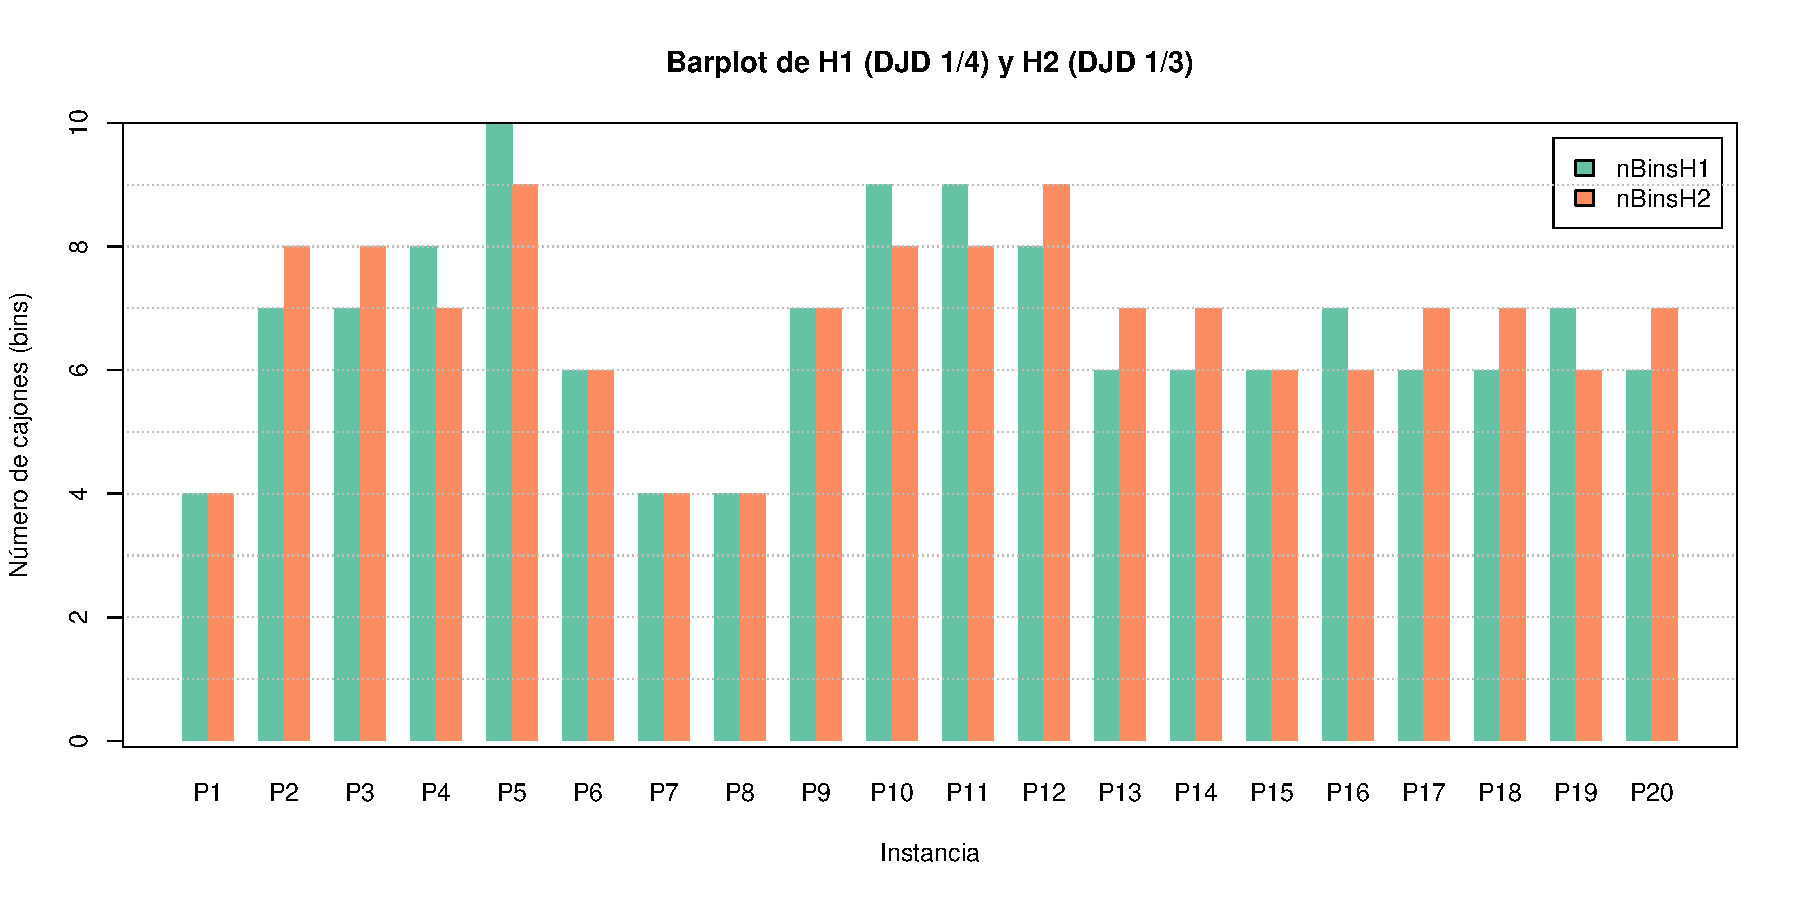
\includegraphics[width=0.8\textwidth]{images/introduction/barplotNumberBinsPerHeuristic}    
    \end{center}  
}
\end{verbatim}
\end{frame}


% new slide
\frame{
  \frametitle{Figure 1 (Output of the previous slide)}
    % add images to the slide
    \begin{center} 
        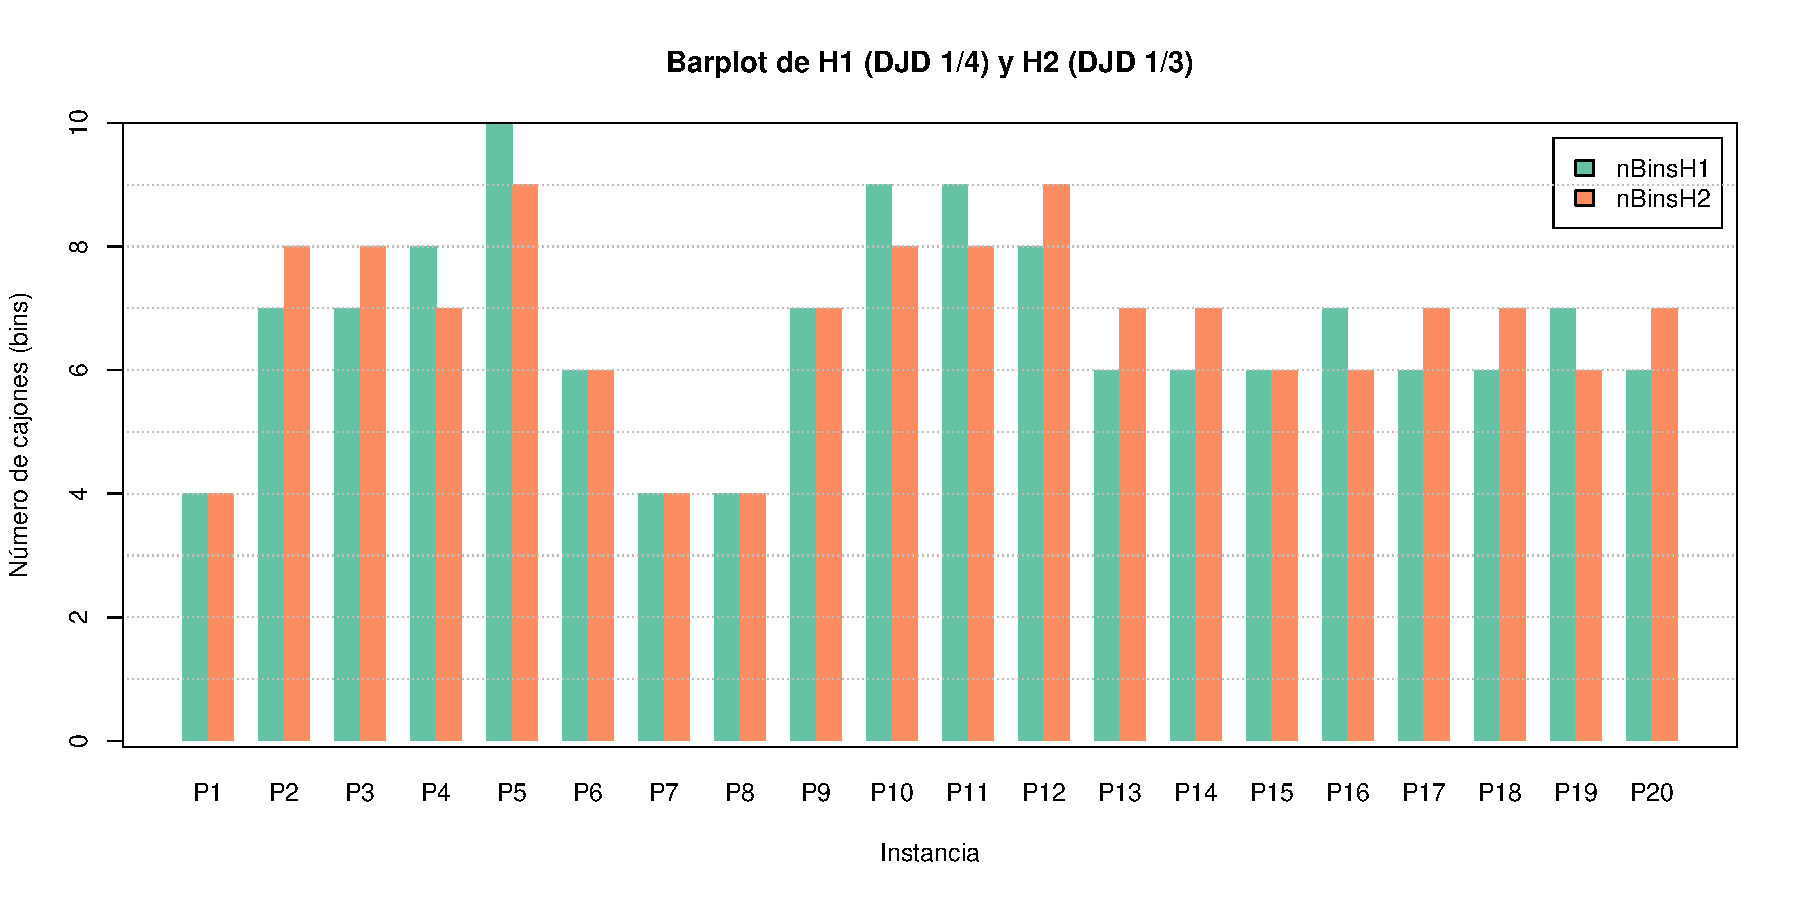
\includegraphics[width=0.99\textwidth]{images/introduction/barplotNumberBinsPerHeuristic}    
    \end{center}  
}

% new slide
\frame{
  \frametitle{Figure 2}
    % add images to the slide
    \begin{center} 
        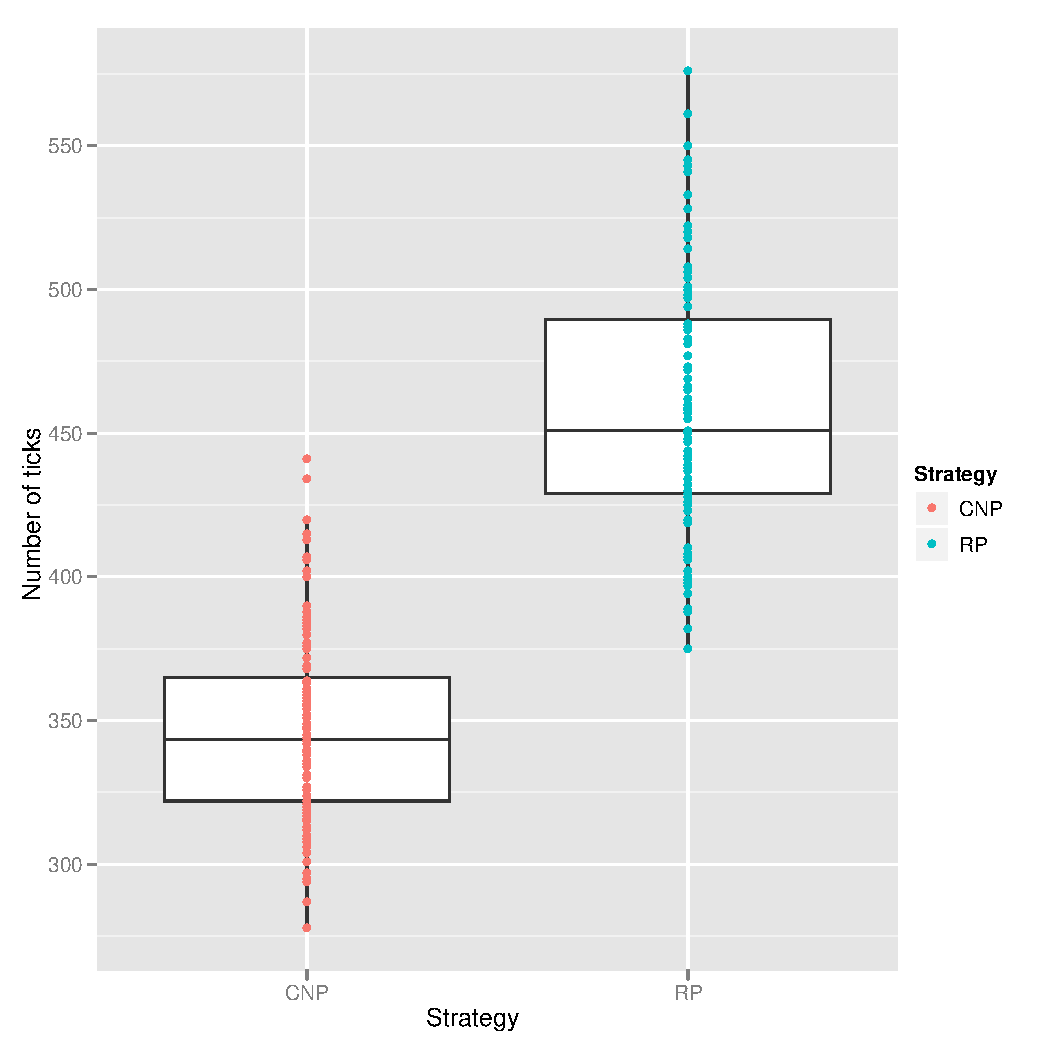
\includegraphics[width=0.6\textwidth]{images/introduction/boxplotTicks}    
    \end{center}  
}

% new slide
\frame{
  \frametitle{Additional notes 1}
       \begin{itemize}
            \item <1-> Please do not forget to take a look at the source code in order to learn how it works
            \item <2-> I've commented the most and critical parts of \textbf{beamerExample.tex} to help in the interpretation of the code
        \end{itemize}
}

% new slide
\frame{
  \frametitle{Additional notes 2}
       \begin{itemize}
            \item <1-> Each .tex file is just to show that you can \textit{split} your presentation into \textbf{sections}
            \item <2-> I prefer to work this way because I find it more organized and with less clutter it boost my understanding of the final PDF file without having to compile a lot of intermediary PDF files
            \item <3-> Always comment your code for further references and I suggest to keep managing your \textbf{sections} as individual .tex files
        \end{itemize}
}

% new slide
\frame{
  \frametitle{More examples | Figure 1}
    % add images to the slide
    \begin{center} 
        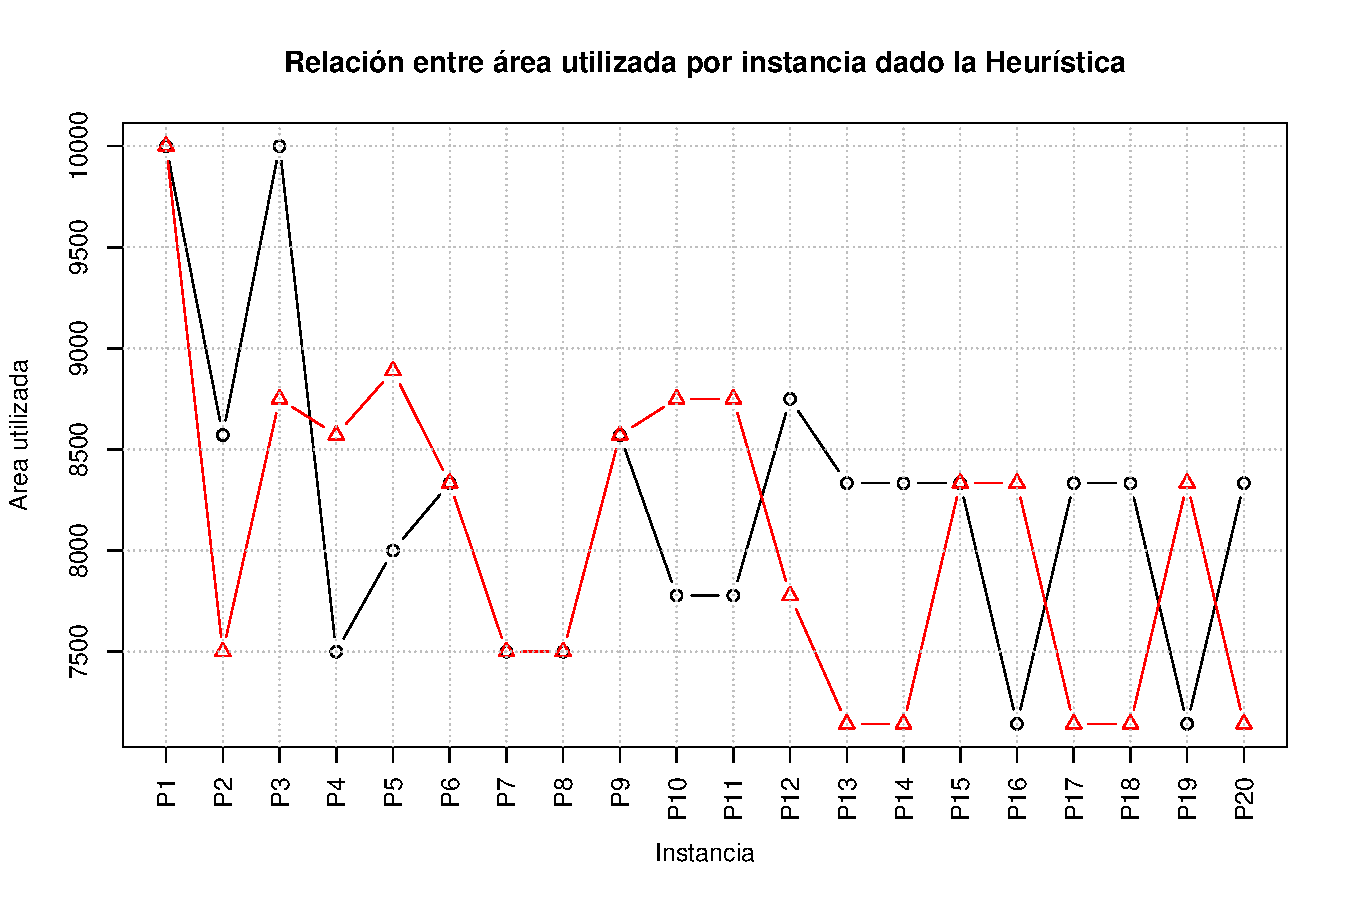
\includegraphics[width=0.9\textwidth]{images/addingImages/matplotAreaUsed}    
    \end{center}  
}

% new slide
\frame{
  \frametitle{More examples | Figure 2}
    % add images to the slide
    \begin{center} 
        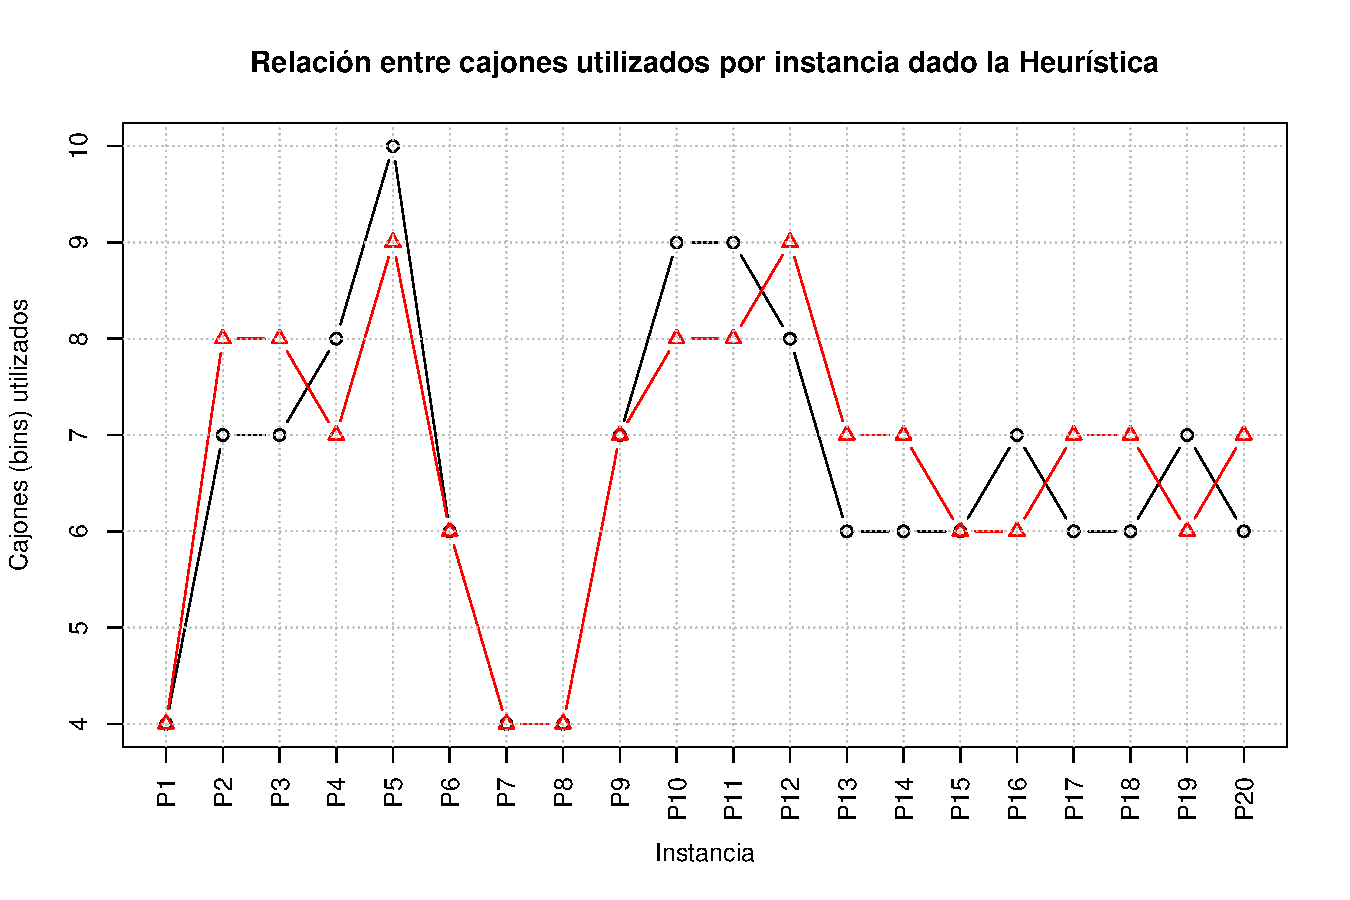
\includegraphics[width=0.9\textwidth]{images/addingImages/matplotNumberOfBins}    
    \end{center}  
}

% new slide
% Comparison of matplotAreaUsed and matplotNumberOfBins
\begin{frame}
    \frametitle{More examples | showing two images in the same slide}
	\begin{columns}[c]
	% FIRST IMAGE
	\column{2.15in}
		\framebox{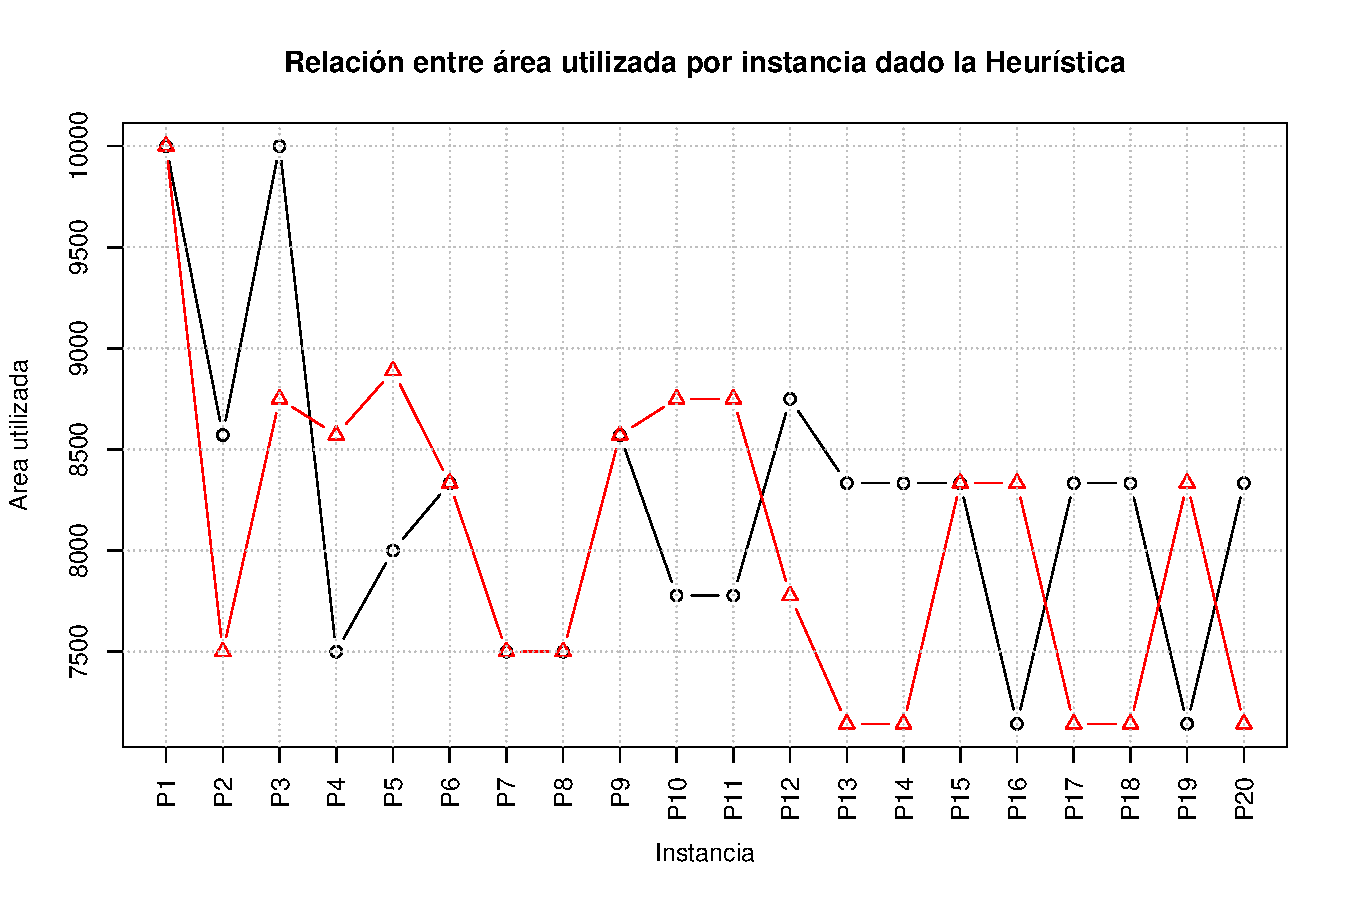
\includegraphics[width=2.2in]{images/addingImages/matplotAreaUsed}}
	% SECOND IMAGE 
	\column{2.4in}
		\framebox{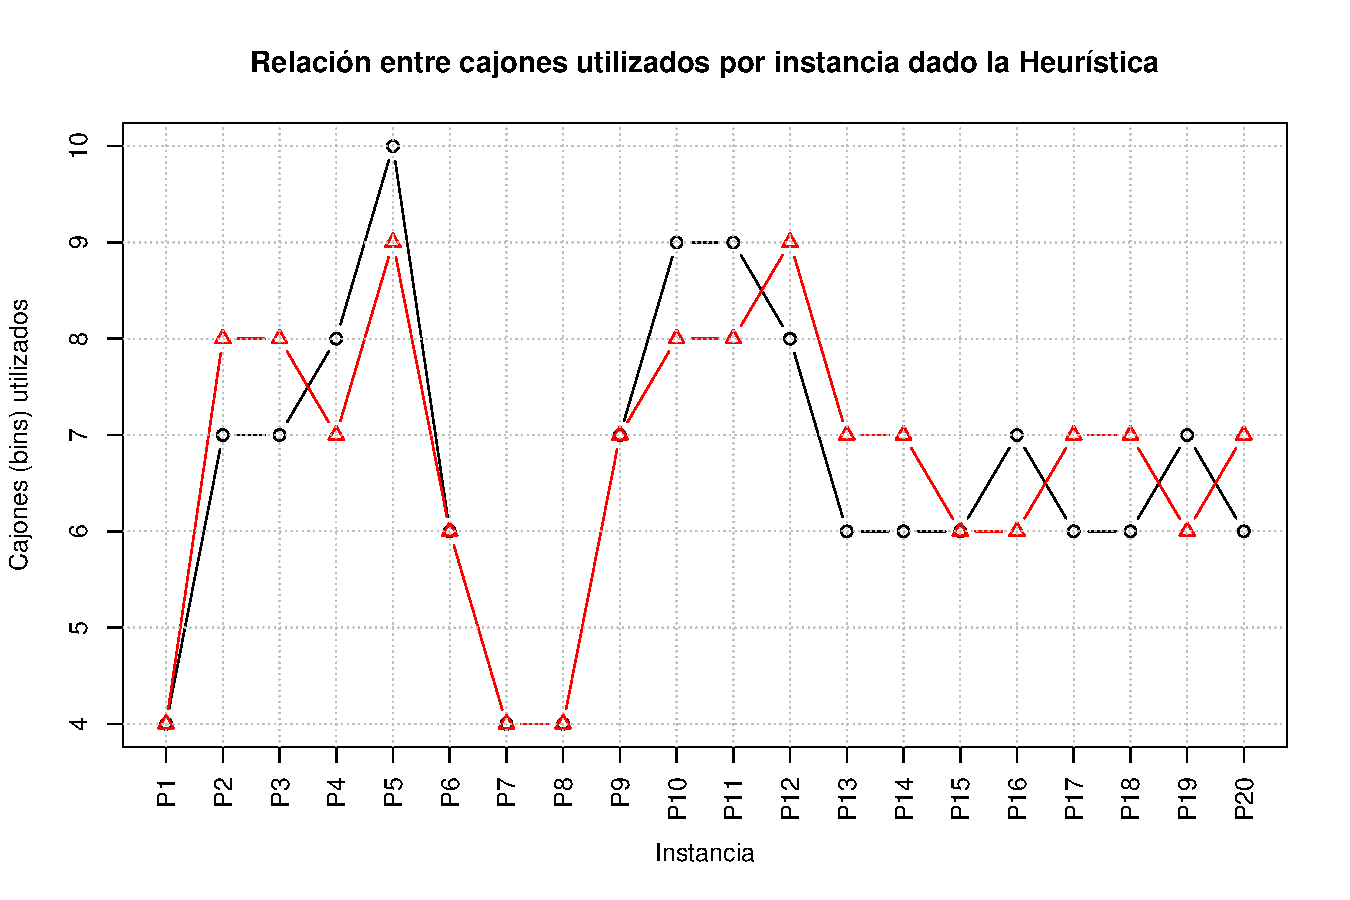
\includegraphics[width=2.2in]{images/addingImages/matplotNumberOfBins}}
	\end{columns}
\end{frame}



% ******************************************************************************
\section{Citing}
% ******************************************************************************

% new slide
\frame{
  \frametitle{Citing inside the document}
       \begin{itemize}
            \item <1-> In this section I will show you how to \textbf{cite} in your presentations
            \item <2-> Please take a look at the source code to see how this works
            \item <3-> I would also recommend you to use \textbf{JabRef} or \textbf{Google Scholar} 
            to retrieve your references in \textbf{BibTex} format
            \item <4-> All the references are placed together in a .bib file
        \end{itemize}
}

% new slide
\begin{frame}[fragile]\small
  \frametitle{BibTex entry format example}
    \begin{verbatim}
@Manual{R2012,
   title        = {R: A Language and Environment 
                   for Statistical
                   Computing},
   author       = {{R Core Team}},
   organization = {R Foundation for Statistical Computing},
   address      = {Vienna, Austria},
   year         = 2012,
   note         = {{ISBN} 3-900051-07-0},
   url          = {http://www.R-project.org}
 }
\end{verbatim}
\end{frame}

% new slide
\frame{
  \frametitle{Compile the document}
       \begin{itemize}
            \item <1-> Do not forget to compile your \TeX{} file at least 3 times (I use the \textbf{pdflatex} command)
            \item <2-> The order I compile this PDF is the following after opening a terminal at the current source directory:
            \begin{itemize}
              \item pdflatex beamerExample
              \item bibtex beamerExample
              \item pdflatex beamerExample
              \item pdflatex beamerExample              
            \end{itemize}
        \end{itemize}
}

% new slide
\begin{frame}[fragile]\small
  \frametitle{Citing inside the document}
    \begin{verbatim}
% new slide
\frame{
\frametitle{Example: Computational tools}
 \begin{itemize}
  \item <1-> Statistical Computing programming 
   language \textbf{R} available 
   at \url{http://cran.r-project.org/} \citep{R2012}
  \item <2-> \textbf{Bioconductor} R packages 
   and tools for the analysis and comprehension 
   of high-throughput genomic data available 
   at \url{http://www.bioconductor.org/} \citep{Gentleman2004}
  \end{itemize}
}
\end{verbatim}
\end{frame}

% new slide
\frame{
  \frametitle{Example: Output of the previous slide}
       \begin{itemize}
            \item <1-> Statistical Computing programming language \textbf{R} available at \url{http://cran.r-project.org/} \citep{R2012}
            \item <2-> \textbf{Bioconductor} R packages and tools for the analysis and comprehension of high-throughput genomic data available at \url{http://www.bioconductor.org/} \citep{Gentleman2004}
        \end{itemize}
}




% ******************************************************************************
\section{Code}
% ******************************************************************************

% new slide
\frame{
  \frametitle{Code}
       \begin{itemize}
            \item <1-> This final section is just to show you how to add \textbf{code} and/or \textbf{equations} in
                        your presentations
        \end{itemize}
}

% new slide
\begin{frame}[t,fragile]{Introduction: Vectors}
    \begin{itemize}
        \item <1-> The basic structure to store data in R
        \item <2-> A vector is a one dimensional array $[a_1,a_2,...,a_n]$
        \item <3-> Common used function of "concatenate" in R: \textbf{c()}\\
        \pause
        \pause
          \vskip1ex
          \verb!x <- c(1,14,16,10)!\\
          \verb! [1] 1 14 16 10!\\
          \pause
          \verb!x <- c("hola","adios","hola de nuevo")!\\
          \verb! [1] "hola" "adios" "hola de nuevo"!\\
          \pause
          \verb!x <- c(TRUE,FALSE,TRUE)!\\
          \verb! [1] TRUE FALSE TRUE!
    \end{itemize}
\end{frame}


% new slide
\begin{frame}[fragile]
   \frametitle{Print code in LaTex using verbatim}
	\begin{verbatim}
for(i in 1:allGenes){
 if(expression[i] > threshold){
   expressed[i] <- gene.id[i]
 }
}
	\end{verbatim}
\end{frame}

% new slide
\begin{frame}[fragile]
   \frametitle{Print code in LaTex using lstlisting}
	\begin{lstlisting}
for(i in 1:allGenes){
 if(expression[i] > threshold){
   expressed[i] <- gene.id[i]
 }
}
	\end{lstlisting}
\end{frame}


% new slide
\frame{
  \frametitle{Print a demo equations}
    \begin{equation}
      x =\frac{-b\pm\sqrt{b^2-4ac}}{2a}
    \end{equation}
    \begin{equation}
      y= \sum_{i=0}^k i^k 
    \end{equation}    
}



% ******************************************************************************
% LOAD BIBLIOGRAPHY
% ******************************************************************************
\begin{frame}[allowframebreaks]{References}
    \bibliographystyle{elsarticle-harv}
    \bibliography{bib/bibliography}
\end{frame}

% ******************************************************************************
% COMPILATION INSTRUCTIONS | RUN IN A TERMINAL
% ******************************************************************************

%	pdflatex beamerExample
%	bibtex beamerExample
%	pdflatex beamerExample
%	pdflatex beamerExample
%	pdflatex beamerExample

%	YES, IT IS NEEDED TO COMPILE THE FILE SEVERAL TIMES BECAUSE
%	LATEX COMPILES LAYER BY LAYER, AT THE FIRST COMPILATION IT WILL DO SOME
%	STUFF AND AT THE SECOND COMPILATION WILL DO ANOTHER STUFF AND SO ON.

\end{document}
